\chapter{Scenarios and Projects}
\label{ch:scenariosprojects}
% ##################################################################################################################

\hfill \textbf{Authors:} Andreas Horni, Benjamin Kickh�fer, Dominik Ziemke

\begin{center} 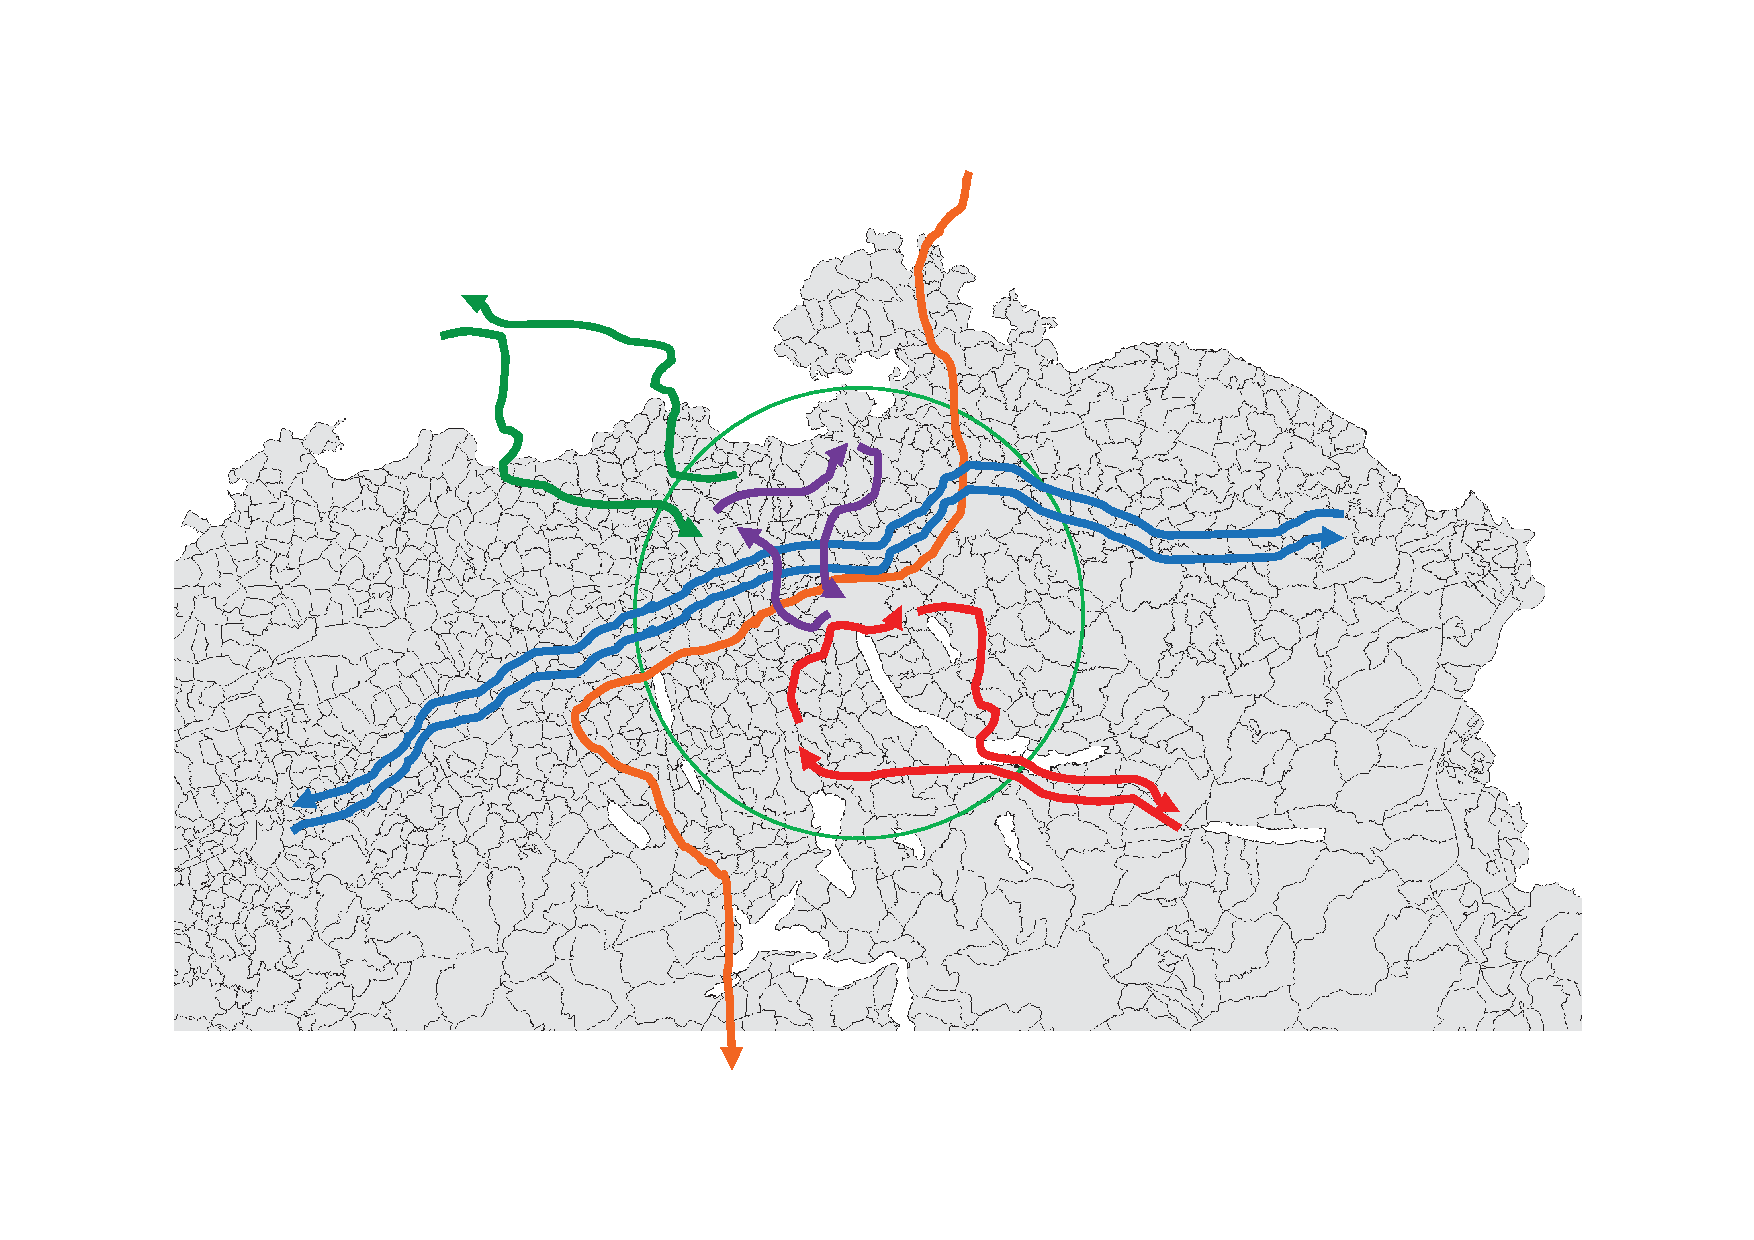
\includegraphics[width=0.7\textwidth, angle=0]{using/figures/zh} \end{center}

% ##################################################################################################################
This chapter summarizes available MATSim scenarios and projects based on MATSim (see also \citet[][]{MATSIM-T-Scenarios_Webpage_2014}). Most scenarios are not public due to privacy issues. However, knowing about the methods used for their creation and problems faced thereby might significantly support the building of new scenarios. 

Scenarios are growing continuously. Here, the latest used version is reported.

Different levels of MATSim involvement are possible. For some regions and projects, MATSim is, for example, only used for traffic assignment whereas for others the complete demand is endogenously handled. Couplings with other forecasting models for transport demand generation have been successfully applied such as the coupling with TASHA for Toronto or the combination of MATSim with the activity-based transport model of Tel Aviv.

% ##################################################################################################################
\section{Scenarios}
This section reports about the study area, demand and supply generation, ...
Utility function is described in Section \ref{sec:utfextensions}.

\ah{Aktuellen Stand von entsprechenden Entwicklern nachfragen/best�tigen lassen.}

%- region description (characteristics, stats, ...)
%- population (popgen, Balmi plug together)
%- facilities
%- network
%- utility function (estimated, how derived)
%- pt (simulated, pseudo pt)
%- modes
%- freight (siehe keynotes Kai)
%- border crossers/boundary effects
%
%data sources
%methods applied
%
%- special problems faced \& solutions found
%
%- simulation quality
%- calibration \& validation (+available data)
%
%- purpose and sponsor/client
%- associated projects -> see Section \ref{sec:projects}
%
%- specialties: parataxis in Gauteng, connections to other sims (Toronto, Tel-Aviv)

% ==================================================================================================================
% ==================================================================================================================
\subsection{Switzerland}
\hfill \textbf{Author:} Andreas Horni

The Switzerland scenario was initially created for the project Westumfahrung (Section \ref{sec:wu}). It serves as the base for the very frequently used Z�rich scenario (Section \ref{sec:zhScenario}). 

Two main branches can be distinguished. The first and older one is based on a one to one translation of the Swiss population census \citep[][]{BfS_VZ_2000}, whereas the second one applies approaches from the family of IPF (Iterative Proportional Fitting) reported by \citet[][]{MuellerKAxhausen_TechRep_IVT_2013, Mueller_unpub_LATSIS_2012, Mueller_unpub_ETC_2011, Mueller_unpub_STRC_2011, Mueller_unpub_IATBR_2012}.

% --------
\paragraph{Associated projects:}
Projects based on the Switzerland scenario are \ah{...}.

% --------
\paragraph{Study area:}
The study area covers all of Switzerland. Due to the administrative borders no data for demand and supply are yet available for the adjoining countries, which can lead to boundary effects. This means that studies focusing on the Swiss border area can not be accomplished to date.

% --------
\paragraph{Population and demand generation:}
The population is derived from the Swiss Census of Population 2000 \citep[][]{BfS_VZ_2000}. The complete Swiss population is modeled which results in around 7.5 million persons. 

Home locations are given at hectare level and work locations are known at municipality level from the commuter matrices, a component of the Swiss Census of Population 2000 \citep[][p.35]{BalmerEtAl_ResRep_bdktzrh_2009}. A very good overview in German of the population generation, its initial individual demand and activity locations can be found in \citet{MeisterEtAl_SVT_2009}. Further information is given in \citet[][]{CiariEtAl_STRC_2008, MeisterEtAl_WCTRS_2010, BalmerEtAl_ResRep_bdktzrh_2009, BalmerEtAl_ResRep_datapuls_2010, BalmerEtAl_HEUREKA_2008}.

The travel demand is basically taken from the National Travel Survey for the years 2000 and 2005 \citep[][]{BfS-MZ2005_manual_2006} (Swiss microcensus). This sample however, substantially underestimates freight traffic and ignores cross-border traffic of non-Swiss residents. Freight traffic for whole of Switzerland is to date missing but border-crossing traffic is added as follows. Cross-border traffic is derived from mode-specific hourly origin-destination matrices given by \citet[][]{VrticEtAl_ResRep_UVEK_2007}, which are disaggregated to around 600'000 individual MATSim plans for all of Switzerland, which contain the cross-border traffic that originates \emph{outside} Switzerland. Non-Swiss cross-border traffic starting in Switzerland is supposed to be negligible. 

% --------
\paragraph{Activity locations:}
The activity location data set, comprising more than $10^6$ home, work, education, shopping and leisure locations, is computed from the Swiss Census of Population 2000 and the Federal Enterprise Census 2001 \citep[][]{SwissEnterpriseCensus_manual_2001} providing hectare level information. In MATSim all locations are termed \emph{activity facilities} or in short \emph{facilities}. The generation of facilities is described in \citet[][p.33]{BalmerEtAl_ResRep_bdktzrh_2009}.

% --------
\paragraph{Network:}
For car traffic the MATSim scenario planning networks and navigation networks from Teleatlas \citep[][]{MultiNet_Webpage_2010} and Navteq \citep[][]{Navteq_2011} have been used. The most often used network is the planning network derived from from the Swiss National Transport Model \citep[][]{VrticEtAl_BiegerEtAl_2003}.

Recently, a network for public transport simulation has been added. It is derived from the National Transport Model of the UVEK described by \citet[][]{VrticFroehlich_ResRep_UVEK_2010}. 

% --------
\paragraph{Modes:}
The scenario simulates car and recently also public transport. The schedules for pt are given at the ``regional'' level. Fine-granular schedules are not yet available. The modes walk and bike are ``teleported''. 

% --------
\paragraph{Calibration and validation:}
Calibration is mainly done for modal split and distance distributions. Utility function values are set accordingly.

For validation count data on city level, cantonal level and national level \citep[][]{ASTRA_Webpage_2006} are available from various sources  resulting in 600 links measured for Switzerland. An average working day (Monday to Thursday, excluding public holidays) is used for comparisons in current projects.

\ah{Simulation quality, achieved results}

% ==================================================================================================================

% ==================================================================================================================
% ##################################################################################################################
\section{Zürich}
\label{sec:zhscenario}
\hfill \textbf{Author:} Andreas Horni

\editdone{This text has undergone the professional edit. Please no grammatical changes anymore! They are most-probably wrong.}

% ##################################################################################################################
The \gls{matsim} team frequently uses the Zürich scenario, based on the Switzerland scenario described above. The Zürich scenario, however, was more detailed; it was enhanced by data available only for the smaller region; e.g., traffic light data or freight demand data was only included for Zürich city and the canton. It is under continuous development, calibration and validation and has been applied in numerous projects, serving as a real-world research example.   

\citet{HorniEtAl_TechRep_IVT_2011_a} provided a technical overview of the first scenario branch; \citet[][]{BalmerEtAl_ResRep_bdktzrh_2009} described its generation for the "Westumfahrung" project . 

The study area was delineated by a circle, with a 30\,kilometer radius around Bellevue, a central and prominent Zürich location. This delineation led to two versions,  the \emph{Zürich diluted scenario} and the \emph{Zürich cut scenario}. For the first, all agents crossing the study area during the simulated day were considered (Figure~\ref{fig:zurichScenario}), resulting in almost 2\,million agents. For the second, only agents remaining in this area the whole day were modeled. The \emph{Zürich cut scenario} was employed as an experiment in \citet[][]{Hackney_PhDThesis_2009}, but using the \emph{Zürich diluted scenario} for production runs is preferable.

Demand was taken directly from the Swiss model; freight traffic was also added to the Zürich scenario, as follows. Canton Zürich raw freight traffic data was taken from the \gls{kvmzh}, provided by \citet{AMV_Webpage_2011} and documented in \citet[][]{GottardiBuergler_SV_1999}.  Zonal level matrices were disaggregated to single \gls{matsim} plans \citep[][]{ShahM_TechRep_IVT_2010}. Matrices for small delivery and heavy trucks were combined into one activity called \emph{freight}. An additional 180\,000 agents were generated for the Zürich region.

For the diluted Zürich scenario, all Swiss facilities, as described above, were used as activity locations. For the diluted scenario, the networks were not thinned out. For  public transport simulation, network and transport schedules were derived from the \gls{kvmzh}. Walk and bike modes were "teleported". 

Calibration was mainly done for modal split and distance distributions and utility function values set accordingly.

For validation, count data on city level, cantonal level and national level \citep[][]{ASTRA_Webpage_2006} were available from various sources, resulting in 123\,links measured for the Zürich  inner city, delineated by a 12\,kilometer radius around Bellevue. The reduced count analysis radius was applied to reduce boundary effects resulting from demand reduction outside the 30\,kilometer radius study area. An average working day (Monday to Thursday, excluding public holidays) was used for comparison in current scenarios.

Some traffic signal data was available for Zürich city \citep[][]{STAPOZH-DAV_unpub_gtZH_2008}; this was integrated for the Westumfahrung project.
%
\createfigure%
{The diluted Zürich scenario}%
{The diluted Zürich scenario}%
{\label{fig:zurichScenario}}%
{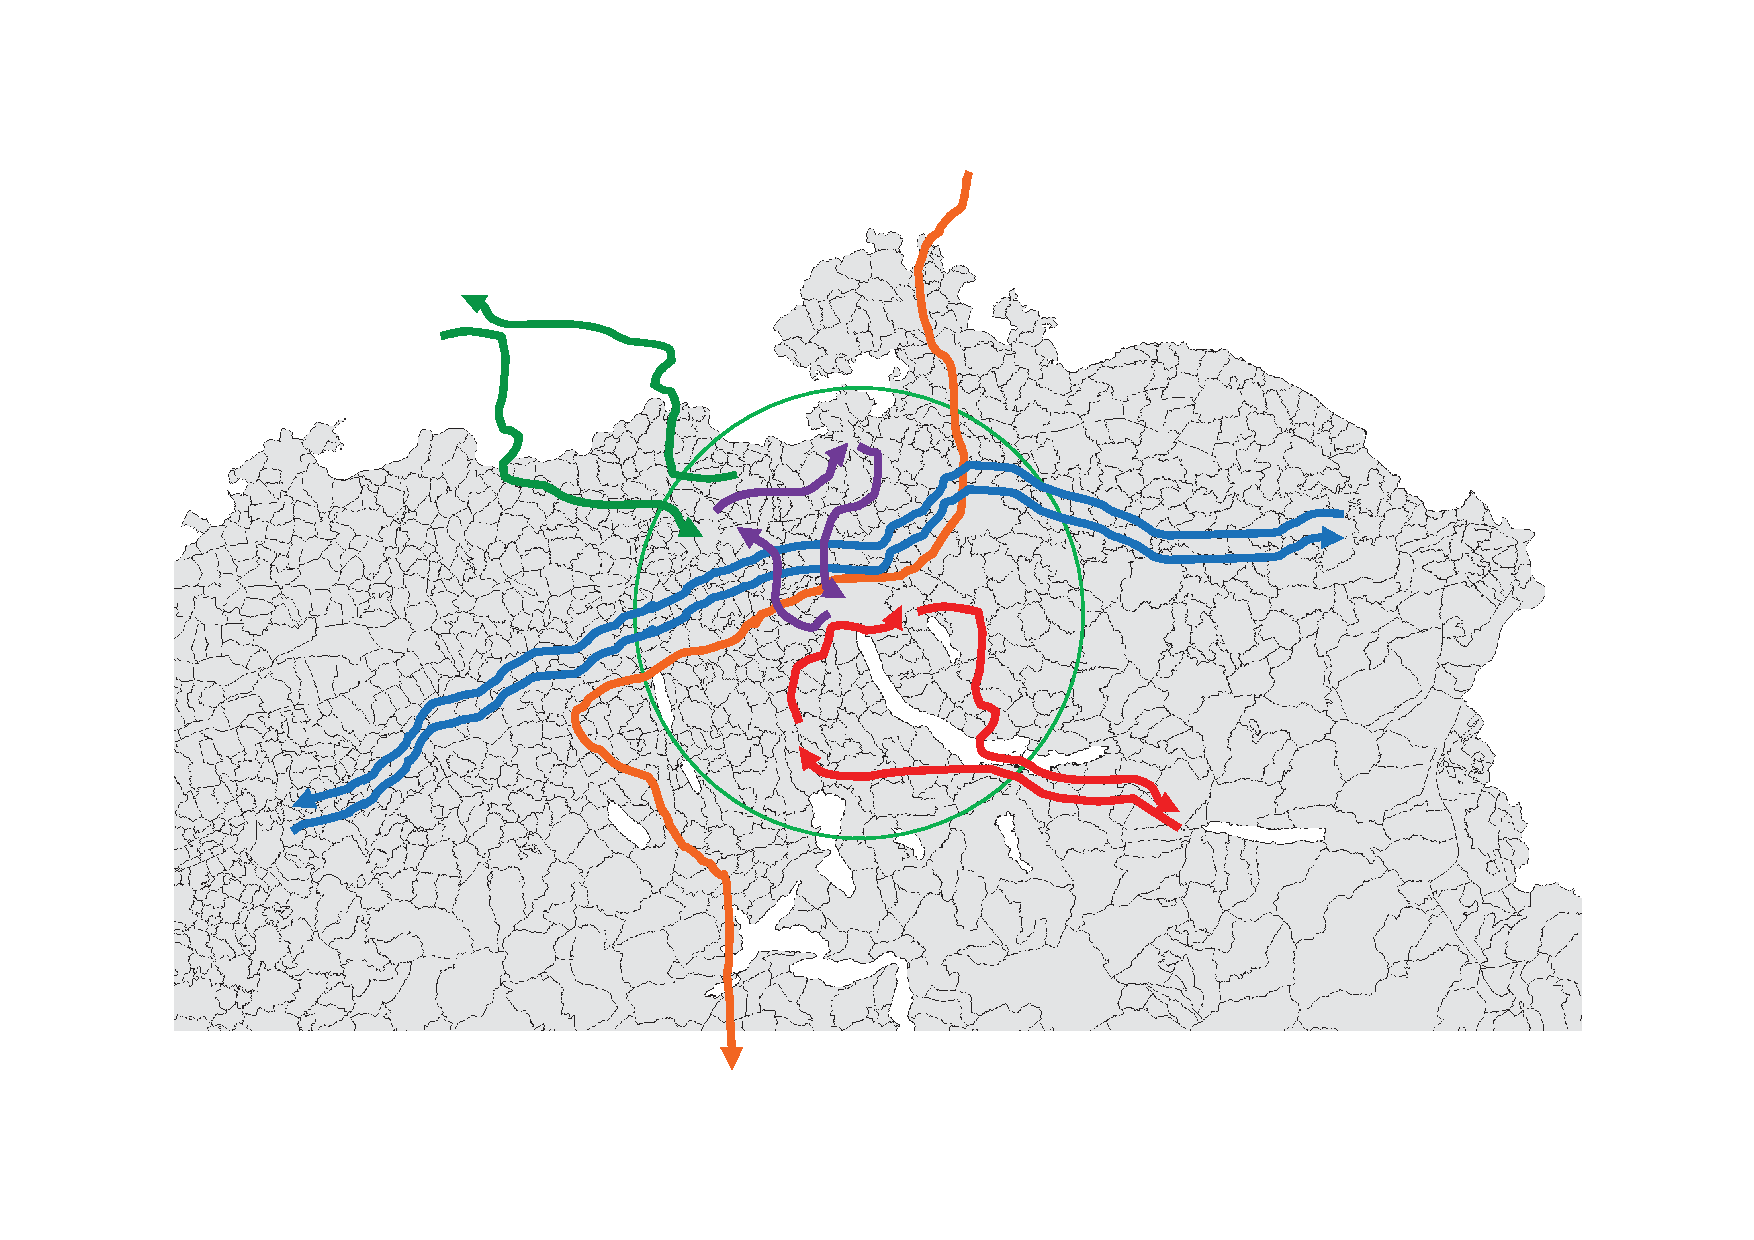
\includegraphics[width=0.99\textwidth, angle=0]{using/figures/zh.pdf}}%
{}

% ##################################################################################################################


% ==================================================================================================================
\subsection{Berlin I: BVG-Scenario \who{Rieser, Neumann}}
\citep[][p.67ff]{Balmer_PhDThesis_2007}

\citep[][Ch 7/8]{Neumann_PhDThesis_2014}

% --------
\paragraph{Associated projects:}

% --------
\paragraph{Study area:}

% --------
\paragraph{Population and demand generation:}

% --------
\paragraph{Activity Locations:}

% --------
\paragraph{Network:}

% --------
\paragraph{Modes:}

% --------
\paragraph{Calibration and validation:}

\ah{Simulation quality, achieved results}

coupling with Visum BVG \\
Marcel: IATBR \\

% ==================================================================================================================
% ##################################################################################################################
\section{Berlin II: CEMDAP-\protect\gls{matsim}-Cadyts Scenario}
\label{sec:berlinII}
\hfill \textbf{Author:} Dominik Ziemke

\editdone{This text has undergone the professional edit. Please no grammatical changes anymore! They are most-probably wrong.}

% ##################################################################################################################
%As explained in section ?????, transport modeling can be considered as the representation of the interaction of transport demand (i.e. people and goods being transported) and transport supply (i.e. transport infrastructure and services) in the transport system. Depending on the application of innovative strategy modules (see section ?????), MATSim accounts for the adaption of transport demand to transport supply \citep{Balmer2007phd}. It is, therefore, crucial to distinguish choice dimensions, which may be adapted during the modeling process (via the application of innovative strategy modules, see section....) and choice dimension whose initial properties are assumed to be correct (e.g. mode shares have to be initially correct in a scenario where the choice of transport modes is not modeled). In the latter case, it is important that respective properties of the transport demand are correct at the start of the simulation (see section Data Requirements - Demand???).
%
To correctly model initial demand properties not included in \gls{matsim} iterations in specific studies (i.e. activity choice), suitable data are needed. Travel diaries containing departure times sequences, mode choice decisions and activity locations are widely used.
%
%A disadvantage of using trip diaries is, however, that all information that is taken from the diaries is by definition not sensitive to policy measures. Also, trip diaries are normally only available for a very small fraction of the population. Another drawback is that, in Germany and the U.S. (and many other parts of the world), the geo-coding of the activity location is considered sensitive information under privacy legislation, and thus increasingly difficult to obtain (cite ZiemkeNagelBhat2015).
However, much of this data source content, particularly location information, is considered sensitive in terms of data privacy legislation and thus increasingly difficult to obtain and process in many areas (e.g.,\,in Germany and the United States) \citep{ZiemkeNagelBhat2015IntegratingCemdapMatsimTransferabilityTRB}.

The \textit{Berlin II scenario} (also referred to as the \emph{CEMDAP-\gls{matsim}-Cadyts scenario} according to applied models in its setup), is the outcome of an alternative approach relying exclusively on freely available and easy-to-obtain input data. Starting points for this scenario are publicly available commuting matrices containing homes and workplaces of workers with social security on the municipality level. Based on this information, it is possible to model morning and evening commuting peaks.

To obtain a full-population demand representation, two further major modeling steps are required. First, in cases like the Berlin case, see below, where commuter matrix spatial resolution is quite coarse, higher resolution \gls{od} information is necessary. Second, a procedure is needed to model secondary activities, i.e.,\,all other activities beyond home and work.

The importance of the first step becomes obvious when looking at the German case; here, the whole city of Berlin, with 3.4\,million inhabitants, is represented by exactly one zone \citep{BA2010Pendlerstatistik}. In the United States, commuting matrices are typically available only on a county-to-county level. Since such location-aggregation-based matrices may become the rule, rather than the exception, in privacy-sensitive societies, a (generalizable) method to attain \gls{od} information at a higher resolution is needed \citep{ZiemkeNagelBhat2015IntegratingCemdapMatsimTransferabilityTRB}. The standard solution would be to estimate an activity location choice model. This, however, is difficult if no trip data to estimate the model is available. \gls{od} matrix estimation studies \citep{ZuylenWillumsenMatrix-from-cnts} suggest that traffic counts may be used to make an initially rough \gls{od} matrix more appropriate for a region. As \gls{matsim} is not based on \gls{od} flows, but on full daily plans, the issue comes down to whether a procedure exists to update these initial full daily plans using traffic counts. In the approach used to create the Berlin II scenario, a procedure proposed by \citet{FloetteroedBierlaireNagel2010Bayesian} and implemented in the software \gls{cadyts}---explained in Chapter~\ref{ch:cadyts})---is applied for this task. Specifically, random draws of possible home and work locations within the home or work municipality given by the commuter matrix are made. Various \gls{matsim} plans, each containing one pair of home and work locations, are created for each agent. Then, the \gls{cadyts} calibration procedure is applied within the iterative \gls{matsim} simulation to select plans and locations more likely to occur with given traffic counts.

As stated above, however, full daily plans (as opposed to mere home-work-home commuting patterns) are needed. Therefore, the second modeling step, the modeling of secondary activities for each individual in the region, needs to be addressed. For the Berlin II scenario, \gls{cemdap} is used to generate initial complete daily plans for each individual. One one hand, however, no \gls{cemdap} parameter set is available for Berlin. On the other hand, and more importantly, one major goal of the study creating the Berlin II scenario was to show its generalizability \citep{ZiemkeNagelBhat2015IntegratingCemdapMatsimTransferabilityTRB}. So, the model parameters of \gls{cemdap} estimated for the Los Angeles region (the estimation context) are retained and then used to generate initial plans for individuals in Berlin (the application context in the current paper), based on Berlin demographic data.

To sum up, home and work municipalities are taken from the commuter matrix. Within these municipalities, a set of (more precisely spatially defined) potential home and work locations are randomly chosen for each agent. Full daily plans incorporating the various potential locations of each agent are generated with \gls{cemdap}, based on a parameter set from another region and local demographic data.

Then, the \gls{cadyts} calibration procedure is used to select those initial full daily plans most consistent with Berlin traffic count data. In other studies, \gls{cadyts} has already been applied to update route choice predictions, both for car \citep{FloetteroedChenEtAl2011BehavioralCalibAndAna} and for public transit \citep{MoyoNagel2013ptNetCalibrationABMTPO}. However, it has not been used to update full daily activity-travel plans, as it was in the procedure that created the Berlin II scenario. 

The Berlin II scenario is an activity-plan-based \gls{matsim} transport model for Berlin based exclusively on freely, or readily, available data. If a commuter matrix, some basic population demographics and traffic counts (or, theoretically, another suitable data source on which to run the calibration procedure) are available for a particular regional context, the approach used to create the Berlin II scenario can be transferred to this context. In fact, the Berlin II scenario itself should be seen as a \emph{transferred model}, because initial plans generated by \gls{cemdap} are based on parameter estimates from another geographic region (the Los Angeles area).

Through a validation based on the Berlin 2008 \gls{srv}, an extensive, regularly-conducted travel survey, the created transport demand representation quality has been successfully tested. So far, the Berlin II scenario exists for a 1\,\% and a 10\,\% population sample of all persons, i.e.,\,including workers without social security, as well as non-working people, aged 18 and above, for the study region. Currently, only motorized traffic is considered. Stability tests, showing that agents' daily plans continue to be chosen when \gls{cadyts} calibration functionality is switched off, have been successfully carried out. This is a clear indication that the scenario is applicable and meaningful for policy studies.

Further improvements, like the addition of public transport and a more realistic representation of the population, are planned. Moreover, similar approaches to integrating activity-travel pattern generators (e.g.,\,the \gls{feathers} model) with \gls{matsim} in transport simulation are planned.

% ##################################################################################################################
%\ah{NOTES: to be removed:
%AN: Szenario entstand aus einer Arbeit zur Nachfragegenerierung. Würde also auch in einen conceptual part passen, anderer Ansatz als die meisten anderen Szenarien ("datensparsam"), Integration von CEMDAP (Modell zur Aktivitätenkettenerzeugung)
%
%Aktivitätenkettenerzeugung: ähnlich zu Tel Aviv Modell
%
%FEATHERS am Beginn -> Vortrag Wiepersdorf
%}

% ##################################################################################################################

% ==================================================================================================================
\subsection{Singapore (Author: ...)}
The Singapore scenario is build at the Future Cities Laboratory in Singapore embedded in the Singapore National Research Foundation initiative CREATE (Campus for Excellence and Technological Enterprise). The scenario is detailed by \citet[][]{ErathEtAl_TechRep_FCL_forth, Erath_unpub_UniSeoul_2011}.

% --------
\paragraph{Associated projects:} 
The scenario is built for the MATSim Singapore project presented in Section \ref{sec:singaporeproject}.

% --------
\paragraph{Study area:} 
The scenario covers the whole republic of Singapore with its approximately 5 million inhabitants.

% --------
\paragraph{Population and demand generation:} 
For population generation an IPF-approach is adopted. A full-population census is not available for Singapore. Demand is derived from a national travel diary survey (Household Interview Travel Survey) reported by \citet[][]{Choi_JOUR_2010} and containing about 11'000 households in Singapore. Home and work locations are assigned by employing a gravity-model-like approach. Freight trips and non-permanent resident inhabitants' trips are generated from origin destination matrices provided by the Singapore Land Transport Authority (LTA).

% --------
\paragraph{Activity Locations:} 
Activity locations are defined at a single building level. Various sources as described in Section 4.1 of \citet[][]{ErathEtAl_TechRep_FCL_forth} have been merged. Workplace capacities are estimated by \citet[][]{OrdonezErath_TRR_2013}. This is required for assigning the fixed activity locations to the agents.

% --------
\paragraph{Network:} 
For the Singapore model both a planning network (provided by LTA) and a Navteq navigation network are readily available. These two networks are combined for the Singapore scenario by a semi-automatic map-matching algorithm. Public transport routes are matched to the network by another map-matching algorithm presented by \citet[][]{Ordonez_HKSTS_2011, Ordonez_Webpage_2011_4}. This enables interaction between public transport and individual traffic.

% --------
\paragraph{Modes:} 
The scenario simulates car and public transport. The modes walk and bike are ``teleported''. Public transport schedules were derived from General Transit Feed Specification (GTFS) created by Google.

% --------
\paragraph{Calibration and validation:}
For validation road count data on an hourly base are available for 200 stations in Singapore.

% --------
\paragraph{Simulation quality and achieved results:}

% --------
\paragraph{Miscellaneous, important to mention:}
Traffic lights are not yet included in the model due to missing data on signal schedules.

% ==================================================================================================================
% ##################################################################################################################
\chapter{Munich}
\label{ch:munich}
\hfill \textbf{Author:} Benjamin Kickhöfer

\editdone{This text has undergone the professional edit. Please no grammatical changes anymore! They are most-probably wrong.}

% ##################################################################################################################
The \gls{matsim} scenario for the Munich metropolitan area was set up during 2010.%
%
\footnote{
%
Detailed descriptions of the scenario can be found in \citet{KickhoeferEtAl_VanoutriveVerhetsel_2013} and \citet{Kickhoefer_PhDThesis_2014}.
%
}
%
The main goal was, and is, simulation of local air pollutant and global greenhouse gas emissions and how their levels change with different policy measures---on aggregated and spatially disaggregated levels. Thus the scenario was used for development and testing of the \gls{emt} (see Chapter~\ref{ch:emissions}). For an example illustrating where overall $\mathit{NO_2}$ private car and freight vehicle emissions are produced over one day, see Figure~\ref{fig:munich:no2emissions}.
%
\createfigure%
{$\mathit{NO_2}$ emissions in Munich}%
{$\mathit{NO_2}$ emissions in Munich}%
{\label{fig:munich:no2emissions}}%
{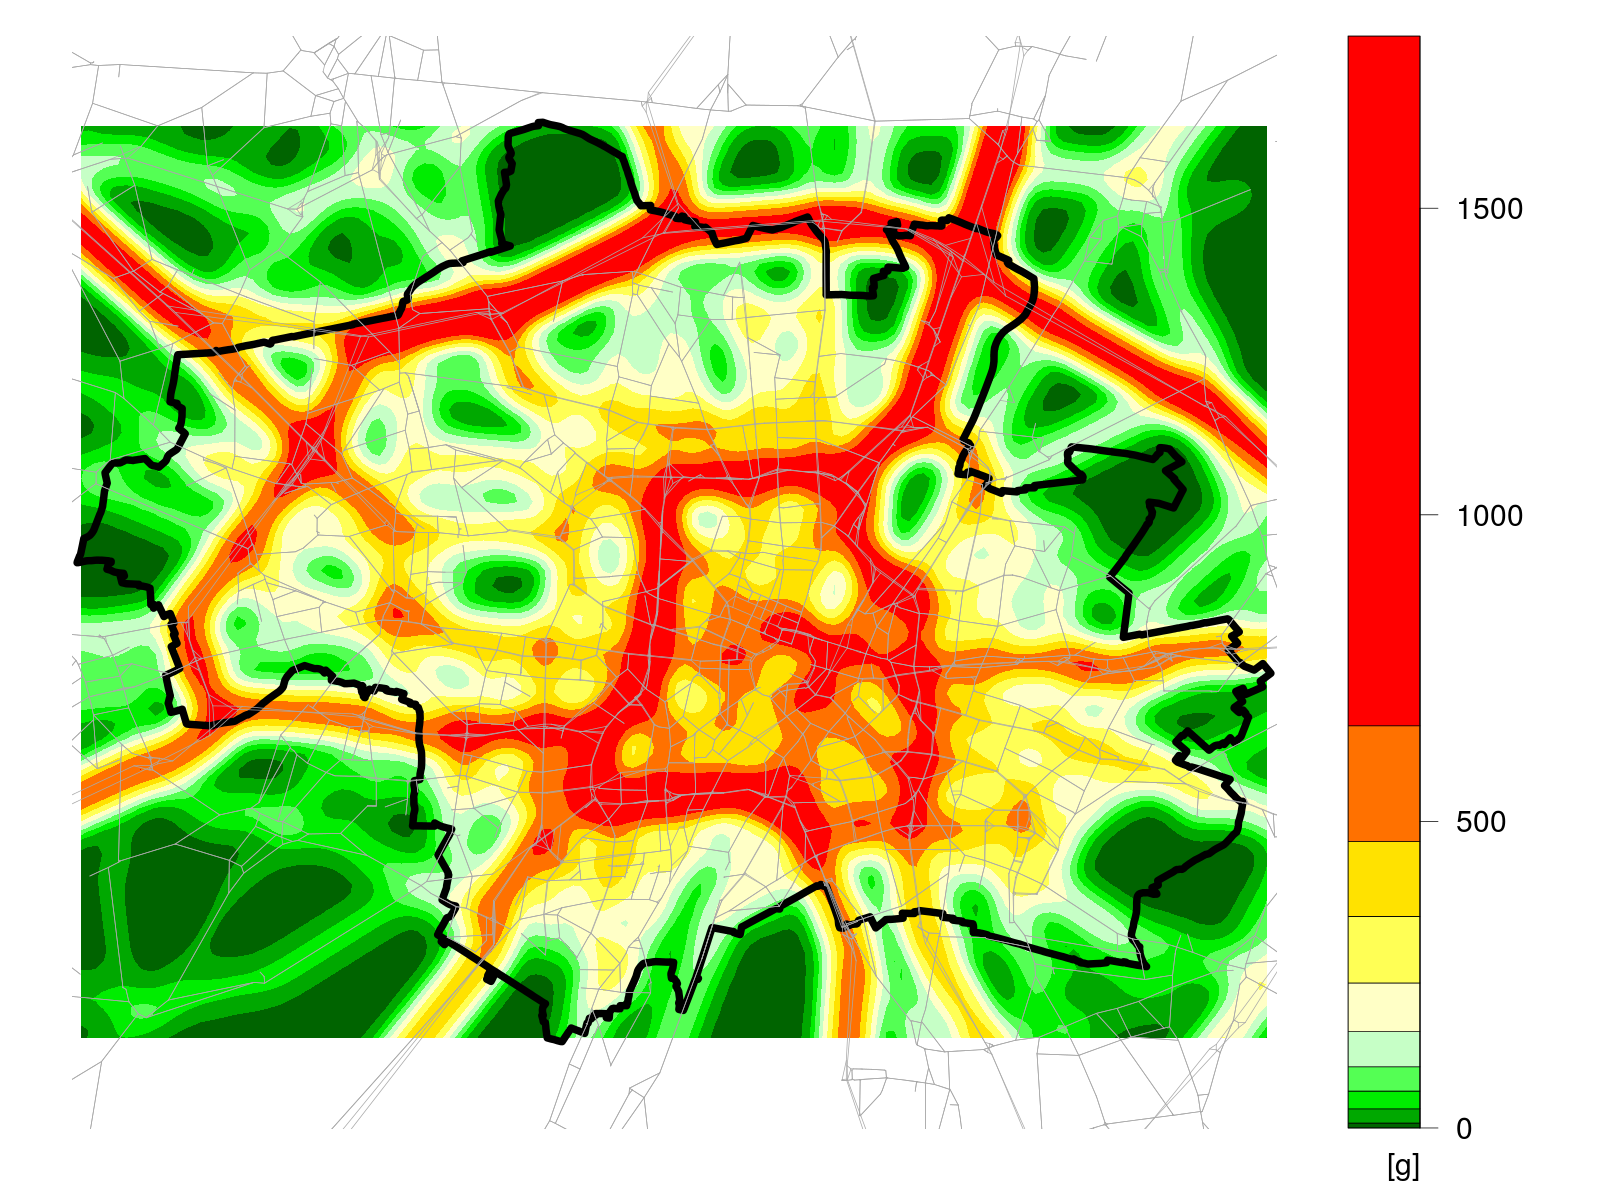
\includegraphics[width=0.85\textwidth, angle=0]{./scenarios/figures/baseCase_1500_NO2_g_108000_0.png}}%
{}

Network information from \acrshort{visum} was converted into \gls{matsim} format, resulting in a network of 17\,888 nodes and 41\,942 links.
%
This transport supply was then linked to travel demand from different sources; an inner-urban traffic activity-based demand from survey data was created, based on \gls{mid} \citep[MiD 2002,][]{FollmerEtAl_TechRep_infasDIW_2004}. This synthetic population segment consisted of roughly 1.4\,million individuals, with detailed vehicle information for every household.
%
Commuters and reverse commuters were modeled with data provided by the German Federal Employment Office \citep{BoehmeEigenhueller_TechRep_IAB_2006}. This part of the population consisted of approximately 0.5\,million individuals, with 0.3\,million commuting to Munich for work. The rest lived in Munich and commuted to their workplace around the city.
%
Freight traffic was also introduced into the model using data from the German Ministry for Transport \citep{ITBBVU_TechRep_2007}. This group consisted of roughly 0.15\,million freight vehicles, performing one commercial trip per day.

The scenario was used for several case studies:
%
\citet{HuelsmannEtAl_LAS_2011} used a single street corridor to validate simulated travel times and emission levels against actual data obtained from a test vehicle.
%
\citet{KickhoeferEtAl_VanoutriveVerhetsel_2013} investigated the relationship between the price elasticities of car travel demand and air pollutant emissions.
%
\citet{HuelsmannEtAl_GerikeEtAl_2013} identified city areas with high air pollution concentration. They defined these areas as ``hotspots'', exceeding the \gls{eu} limits for \gls{no2}. The authors raised toll levels incrementally for vehicles passing these hotspots, until high pollution concentrations disappeared, to estimate true threshold value \gls{eu} avoidance costs.
%
\citet{KickhoeferNagel2012EmissionInternalization} derived time-dependent, vehicle-specific, first-best air pollution tolls to create a benchmark for real-world policy evaluation.
%
\citet{KickhoeferKern_MobilTUM_2014} went one step further and calculated time-dependent, vehicle-specific air pollution exposure tolls to correct toll levels with \citet{KickhoeferNagel2012EmissionInternalization} for a count of individuals affected.



% ##################################################################################################################

% ==================================================================================================================
\subsection{City of Sioux Falls (South Dakota)}

Often used test scenario \citep[][]{BarGera_TNTP_Webpage_2013}. Not aimed at replicating the real City of Sioux Falls, South Dakota.
reported at www.matsim.org/scenario/sioux-falls.
and in \citet[][]{ChakirovFourie_TechRep_FCL_2014}.


% --------
\paragraph{Associated projects:} 

% --------
\paragraph{Study area:} City of Sioux Falls

% --------
\paragraph{Population and demand generation:}
synthetic populaltion generation based on PUS adopting the synthetic reconstruction method.

demand
derived from real microcensus from the real city of Sioux falls

only 2 chains: home-work-home and home-other-home.

destinations using a parameter-free radiation model as introduced by \citet[][]{SiminiEtAl_NAT_2012}.

% --------
\paragraph{Activity Locations:} data set of buildings provided by the City of Sioux Falls GIS division.

% --------
\paragraph{Network:} adding bus network. adjusting network to make it dynamic.

% --------
\paragraph{Modes:}

% --------
\paragraph{Calibration and validation:}

% --------
\paragraph{Simulation quality and achieved results:}

% --------
\paragraph{Miscellaneous, important to mention:}


% ==================================================================================================================
\subsection{Gauteng}
\citep[][]{JoubertJEtAl_TRR_2010}

% --------
\paragraph{Associated projects:}

% --------
\paragraph{Study area:}

% --------
\paragraph{Population and demand generation:}

% --------
\paragraph{Activity Locations:}

% --------
\paragraph{Network:}

% --------
\paragraph{Modes:}

% --------
\paragraph{Calibration and validation:}

\ah{Simulation quality, achieved results}

% ==================================================================================================================
\subsection{Padang}
\citep[][]{Laemmel_PhDThesis_2011}

% --------
\paragraph{Associated projects:}

% --------
\paragraph{Study area:}

% --------
\paragraph{Population and demand generation:}

% --------
\paragraph{Activity Locations:}

% --------
\paragraph{Network:}

% --------
\paragraph{Modes:}

% --------
\paragraph{Calibration and validation:}

\ah{Simulation quality, achieved results}

% ==================================================================================================================
\subsection{Shanghai}
\citep[][]{WangtEtAl_TRB_2013}

% --------
\paragraph{Associated projects:}

% --------
\paragraph{Study area:}

% --------
\paragraph{Population and demand generation:}

% --------
\paragraph{Activity Locations:}

% --------
\paragraph{Network:}

% --------
\paragraph{Modes:}

% --------
\paragraph{Calibration and validation:}

\ah{Simulation quality, achieved results}

% ==================================================================================================================
\subsection{Toronto \who{Balmer}}
\citep[][]{GaoWEtAl_TRR_2010}

coupling with TASHA

% --------
\paragraph{Associated projects:}

% --------
\paragraph{Study area:}

% --------
\paragraph{Population and demand generation:}

% --------
\paragraph{Activity Locations:}

% --------
\paragraph{Network:}

% --------
\paragraph{Modes:}

% --------
\paragraph{Calibration and validation:}

\ah{Simulation quality, achieved results}

% ==================================================================================================================
\subsection{Tel Aviv \who{Dobler}}
\label{sec:telavivScenario}
\citep[][]{BekhorEtAl_TRB_2011}

% --------
\paragraph{Associated projects:}

% --------
\paragraph{Study area:}

% --------
\paragraph{Population and demand generation:}

% --------
\paragraph{Activity Locations:}

% --------
\paragraph{Network:}

% --------
\paragraph{Modes:}

% --------
\paragraph{Calibration and validation:}

\ah{Simulation quality, achieved results}

% ==================================================================================================================
\subsection{Poznan \who{Maciejewski}}

% --------
\paragraph{Associated projects:}

% --------
\paragraph{Study area:}

% --------
\paragraph{Population and demand generation:}

% --------
\paragraph{Activity Locations:}

% --------
\paragraph{Network:}

% --------
\paragraph{Modes:}

% --------
\paragraph{Calibration and validation:}

\ah{Simulation quality, achieved results}

% ==================================================================================================================
\subsection{Cottbus \who{Bischoff}}
AN-Mail: frei verf�gbar. �V vorhanden, 100\% Szenario, das sich mit einigermassen geringem Aufwand rechnen l�sst. Grundlage f�r Dominik G.s Ampelpart


% ==================================================================================================================
\subsection{Los Angeles \who{Goulias, Balmer}}
Los Angeles 107 CEMDAP MATSim -

% ==================================================================================================================
\subsection{Patna \who{Agarwal}}

% ==================================================================================================================
\subsection{Rotterdam (Milan Lovric, Bouman)}

% ==================================================================================================================
Further models are currently being developed \citep[][]{Axhausen_unpub_Hong_Kong_2013} for the Netherlands (coupled with Albtratross (by whom? Dobi?), Cape Town, London, Seoul, Dublin, and New York \citep[][]{Balmer_unpub_ZMNY_2014}.

Chicago? -> Wiepersdorf

% ##################################################################################################################
